\documentclass[mathserif, xcolor=table, svgnames]{beamer}
\mode<presentation>
{
  \usetheme{Hannover}
  \setbeamercovered{transparent}
}
\usepackage[english]{babel}
\usepackage[utf8]{inputenc}
\usepackage[T1]{fontenc}
\usepackage{amsthm}
\usepackage{array,xspace}
\usepackage{dcolumn}
\usepackage{eulervm}
\usepackage{eurosym}
\usepackage{graphicx}
\usepackage{booktabs, multicol, multirow}
\usepackage{relsize}
\usepackage{wasysym}

\input{isomath.tex}
\colorlet{OurColor}{LawnGreen!40}
\colorlet{ShadedRowColor}{LightSkyBlue!40}

\newcommand{\eur}{\EUR{}}
\newcommand{\individuals}{\mathbbm{I}}
\newtheorem{proposition}{Proposition}
\newcommand{\std}[1]{\small\color{lightgray}{#1}}
\long\def\GobbleColumnStart#1\GobbleColumnStop{}
\let\GobbleColumnStop\relax
\newcolumntype{i}{>{\GobbleColumnStart}c<{\GobbleColumnStop}}
\newcommand{\V}{\ensuremath{\surd}}
\newcommand{\YSM}{\ensuremath{\text{YSM}}\xspace}
\graphicspath{{./}{cartoons/}{images/}}

\title{Introduction to Apache Spark}
\author{Ott Toomet}
\date{Computational Demography\\
2017-02-16}

\begin{document}
\setkeys{Gin}{width=\textwidth}

\begin{frame}
  \maketitle
\end{frame}

\section{What is Spark}

\begin{frame}
  \frametitle{What is Apache Spark}
  \begin{itemize}
  \item In-memory cluster computing
    \begin{itemize}
    \item Shuffles around code, not data
    \end{itemize}
  \item Can use various data sources (including distributed file
    systems, databases)
  \item Includes \emph{MapReduce} framework (like Hadoop)
  \item Also includes advanced processing, ML
  \item Popular and rapidly developing
  \end{itemize}
\end{frame}

\begin{frame}
  \frametitle{Components}
  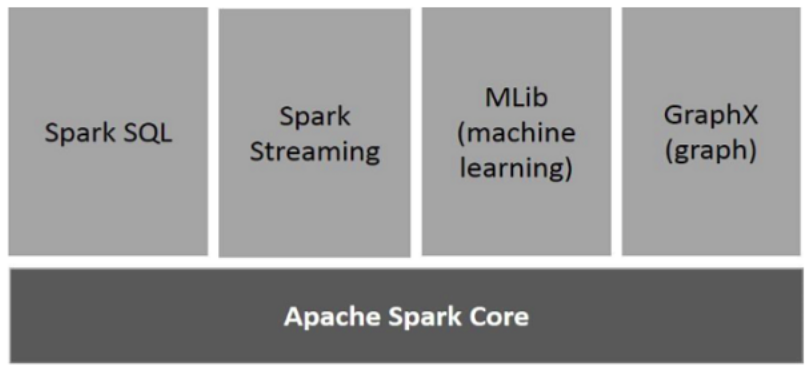
\includegraphics{components_of_spark.png}
\end{frame}

\begin{frame}
  \frametitle{Spark Core}
  \begin{itemize}
  \item 1 Driver + many executors
    \begin{itemize}
    \item Executors may be on different nodes
    \item Related memory needs
    \end{itemize}
  \item Written in scala
    \begin{itemize}
    \item API for scala, java, python, R
    \end{itemize}
  \item RDD: Resilient Distributed Dataset
    \begin{itemize}
    \item Distributed: partitioned across the spark cluster
    \item Resilient: if a partition fails, only that partition is
      recovered
    \end{itemize}
  \item Lazy evaluation
    \begin{itemize}
    \item Postpone hard computations as long as possible
    \end{itemize}
  \end{itemize}
\end{frame}

\begin{frame}
  \frametitle{Components}
  \begin{itemize}
  \item Spark SQL
    \begin{itemize}
    \item DataFrames (R API)
    \item SQL interface
      \begin{itemize}
      \item Use standard SQL queries
      \end{itemize}
    \end{itemize}
  \item Spark Streaming
    \begin{itemize}
    \item Real-time input, real-time output
    \item Made of RDD-s
    \end{itemize}
  \item Spark ML
    \begin{itemize}
    \item Collection of ML algorithms
    \end{itemize}
  \item graphX
    \begin{itemize}
    \item Graph data structure
    \end{itemize}
  \end{itemize}
\end{frame}

\begin{frame}
  \frametitle{Conclusion}
  \begin{itemize}
  \item Allows to access big datasets
    \begin{itemize}
    \item Sometimes works rather well
    \item Sometimes extremely hard to get to work
    \end{itemize}
  \item Documentations is \emph{bad}
    \begin{itemize}
    \item Even Stackoverflow not too helpful
    \end{itemize}
  \item Feels to be in the beta stage
    \begin{itemize}
    \item Bugs, functionality missing, etc
    \item Is this what bleeding edge means?
    \end{itemize}
  \end{itemize}
\end{frame}

\end{document}
